% generated by ledger -- do not edit; run `ledger figures`
% metrics_hash: 53a2534632050563e91e74856e470557fe8b2df54f7c4514e6ed2c5985302d8d
%% requires \usepackage{pgfplots} in the preamble
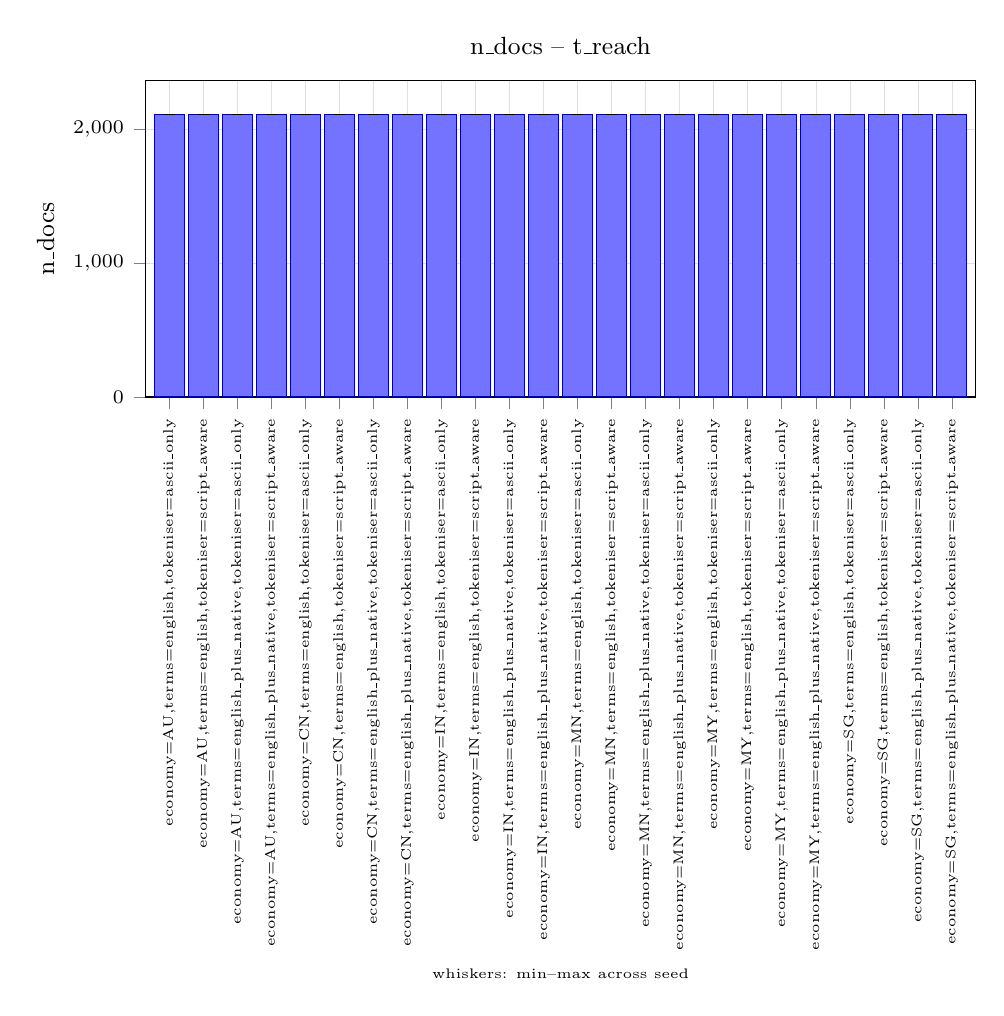
\begin{tikzpicture}
\begin{axis}[
  ybar, width=\linewidth, height=5.6cm,
  ymin=0.000000, ymax=2366.560000,
  xmin=-0.7, xmax=23.7,
  bar width=10.83pt,
  xtick=data, xticklabels={{economy=AU,terms=english,tokeniser=ascii\_only},{economy=AU,terms=english,tokeniser=script\_aware},{economy=AU,terms=english\_plus\_native,tokeniser=ascii\_only},{economy=AU,terms=english\_plus\_native,tokeniser=script\_aware},{economy=CN,terms=english,tokeniser=ascii\_only},{economy=CN,terms=english,tokeniser=script\_aware},{economy=CN,terms=english\_plus\_native,tokeniser=ascii\_only},{economy=CN,terms=english\_plus\_native,tokeniser=script\_aware},{economy=IN,terms=english,tokeniser=ascii\_only},{economy=IN,terms=english,tokeniser=script\_aware},{economy=IN,terms=english\_plus\_native,tokeniser=ascii\_only},{economy=IN,terms=english\_plus\_native,tokeniser=script\_aware},{economy=MN,terms=english,tokeniser=ascii\_only},{economy=MN,terms=english,tokeniser=script\_aware},{economy=MN,terms=english\_plus\_native,tokeniser=ascii\_only},{economy=MN,terms=english\_plus\_native,tokeniser=script\_aware},{economy=MY,terms=english,tokeniser=ascii\_only},{economy=MY,terms=english,tokeniser=script\_aware},{economy=MY,terms=english\_plus\_native,tokeniser=ascii\_only},{economy=MY,terms=english\_plus\_native,tokeniser=script\_aware},{economy=SG,terms=english,tokeniser=ascii\_only},{economy=SG,terms=english,tokeniser=script\_aware},{economy=SG,terms=english\_plus\_native,tokeniser=ascii\_only},{economy=SG,terms=english\_plus\_native,tokeniser=script\_aware}},
  x tick label style={rotate=90, anchor=east, font=\tiny},
  y tick label style={font=\scriptsize},
  ylabel={n\_docs}, ylabel style={font=\small},
  title={n\_docs -- t\_reach}, title style={font=\small},
  xlabel={whiskers: min--max across seed}, xlabel style={font=\tiny},
  grid=major, grid style={very thin, gray!25},
  tick align=outside, tick pos=left,
]
\addplot+[ybar, fill=blue!55, draw=blue!70!black,
  error bars/.cd, y dir=both, y explicit,
  error bar style={black, thin}] table[x=i, y=mean,
  y error plus=eplus, y error minus=eminus] {
i mean eplus eminus
0 2113.000000 0.000000 0.000000
1 2113.000000 0.000000 0.000000
2 2113.000000 0.000000 0.000000
3 2113.000000 0.000000 0.000000
4 2113.000000 0.000000 0.000000
5 2113.000000 0.000000 0.000000
6 2113.000000 0.000000 0.000000
7 2113.000000 0.000000 0.000000
8 2113.000000 0.000000 0.000000
9 2113.000000 0.000000 0.000000
10 2113.000000 0.000000 0.000000
11 2113.000000 0.000000 0.000000
12 2113.000000 0.000000 0.000000
13 2113.000000 0.000000 0.000000
14 2113.000000 0.000000 0.000000
15 2113.000000 0.000000 0.000000
16 2113.000000 0.000000 0.000000
17 2113.000000 0.000000 0.000000
18 2113.000000 0.000000 0.000000
19 2113.000000 0.000000 0.000000
20 2113.000000 0.000000 0.000000
21 2113.000000 0.000000 0.000000
22 2113.000000 0.000000 0.000000
23 2113.000000 0.000000 0.000000
};
\end{axis}
\end{tikzpicture}
